\documentclass{standalone}
\usepackage[dvipsnames]{xcolor}
\usepackage{tikz}
\usetikzlibrary{calc,matrix,positioning,fit,backgrounds}

\colorlet{region}{Melon}
\colorlet{complement}{SkyBlue}
\colorlet{border}{LimeGreen}

\newcommand{\pucond}{$p^{cond}_{\uparrow}$}
\newcommand{\pdcond}{$p^{cond}_{\downarrow}$}

\begin{document}
\pgfdeclarelayer{bg}
\pgfdeclarelayer{grid}
\pgfsetlayers{bg,grid,main}

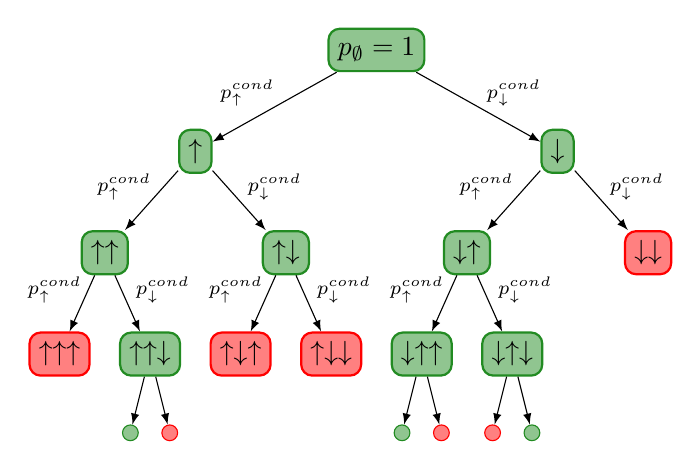
\begin{tikzpicture}[
      level 1/.style={sibling distance=4.6cm},
      level 2/.style={sibling distance=2.3cm},
      level 3/.style={sibling distance=1.15cm},
      level 4/.style={sibling distance=5mm},
      nonleaf/.style={draw,thick,rounded corners,anchor=north},
      leaf/.style={circle, minimum width=2mm,inner sep=0, fill},
      accept/.style={draw=ForestGreen, fill=ForestGreen!50!white},
      drop/.style={draw=red, fill=red!50!white},
      edge from parent/.style={draw,-latex},
      label/.style={inner sep=0,font={\scriptsize}},
      rlab/.style={label,right=1mm,anchor=south west},
      llab/.style={label,left=0,anchor=south east},
      level distance=1cm
  ]
  \node[nonleaf, accept] {$p_{\emptyset}=1$}
  child {
    node[nonleaf, accept] {$\uparrow$}
    child {
      node[nonleaf, accept] {$\uparrow\uparrow$}
      child {
        node[nonleaf, drop] {$\uparrow\uparrow\uparrow$}
        edge from parent node[llab] {\pucond}
      }
      child {
        node[nonleaf, accept] {$\uparrow\uparrow\downarrow$}
        child {
          node[leaf, accept] {}
        }
        child {
          node[leaf, drop] {}
        }
        edge from parent node[rlab] {\pdcond}
      }
      edge from parent node[llab] {\pucond}
    }
    child {
      node[nonleaf, accept] {$\uparrow\downarrow$}
      child {
        node[nonleaf, drop] {$\uparrow\downarrow\uparrow$}
        edge from parent node[llab] {\pucond}
      }
      child {
        node[nonleaf, drop] {$\uparrow\downarrow\downarrow$}
        edge from parent node[rlab] {\pdcond}
      }
      edge from parent node[rlab] {\pdcond}
    }
    edge from parent node[llab] {\pucond}
  }
  child {
    node[nonleaf, accept] {$\downarrow$}
    child {
      node[nonleaf, accept] {$\downarrow\uparrow$}
      child {
        node[nonleaf, accept] {$\downarrow\uparrow\uparrow$}
        child {
          node[leaf, accept] {}
        }
        child {
          node[leaf, drop] {}
        }
        edge from parent node[llab] {\pucond}
      }
      child {
        node[nonleaf, accept] {$\downarrow\uparrow\downarrow$}
        child {
          node[leaf, drop] {}
        }
        child {
          node[leaf, accept] {}
        }
        edge from parent node[rlab] {\pdcond}
      }
      edge from parent node[llab] {\pucond}
    }
    child {
      node[nonleaf, drop] {$\downarrow\downarrow$}
      edge from parent node[rlab] {\pdcond}
    }
    edge from parent node[rlab] {\pdcond}
  };

\end{tikzpicture}
\end{document}
